
% Copyright 2004 by Till Tantau <tantau@users.sourceforge.net>.
%
% In principle, this file can be redistributed and/or modified under
% the terms of the GNU Public License, version 2.
%
% However, this file is supposed to be a template to be modified
% for your own needs. For this reason, if you use this file as a
% template and not specifically distribute it as part of a another
% package/program, I grant the extra permission to freely copy and
% modify this file as you see fit and even to delete this copyright
% notice. 

\documentclass[pdf]{beamer}
\mode<presentation>{}

\usepackage[utf8]{inputenc}
\usepackage{amssymb}
\usepackage{amsmath}
\usepackage{graphicx}


% There are many different themes available for Beamer. A comprehensive
% list with examples is given here:
% http://deic.uab.es/~iblanes/beamer_gallery/index_by_theme.html
% You can uncomment the themes below if you would like to use a different
% one:
%\usetheme{AnnArbor}
%\usetheme{Antibes}
%\usetheme{Bergen}
%\usetheme{Berkeley}
%\usetheme{Berlin}
%\usetheme{Boadilla}
%\usetheme{boxes}
%\usetheme{CambridgeUS}
\usetheme{Copenhagen}
%\usetheme{Darmstadt}
%\usetheme{default}
%\usetheme{Frankfurt}
%\usetheme{Goettingen}
%\usetheme{Hannover}
%\usetheme{Ilmenau}
%\usetheme{JuanLesPins}
%\usetheme{Luebeck}
%\usetheme{Madrid}
%\usetheme{Malmoe}
%\usetheme{Marburg}
%\usetheme{Montpellier}
%\usetheme{PaloAlto}
%\usetheme{Pittsburgh}
%\usetheme{Rochester}
%\usetheme{Singapore}
%\usetheme{Szeged}
%\usetheme{Warsaw}
%\usecolortheme{seahorse}


\title{Orthogonal Range Searching in $2$D\\ using Ball Inheritance}
\author{Mads Ravn}
\institute{Computer Science, Aarhus University}
\date{2015}
 
\pgfdeclareimage[height=0.5cm]{university-logo}{logo-eps-converted-to.pdf}
\logo{\pgfuseimage{university-logo}}

% Delete this, if you do not want the table of contents to pop up at
% the beginning of each subsection:
\AtBeginSubsection[]
{
  \begin{frame}<beamer>{Outline}
    \tableofcontents[currentsection,currentsubsection]
  \end{frame}
}

% Let's get started
\begin{document}

\begin{frame}
  \titlepage
\end{frame}

\begin{frame}
  \begin{itemize}
    \item Giv en præsentation af den i specialet introducerede simplificerede datastruktur til range searching i 2d. (3)
    \item Beskriv ball-inheritance problemet og forklar sammenhængen til range searching. (2)
    \item Beskriv også det klassiske kd-træ (1)
    \item og fortæl om hvilke eksperimenter du har foretaget for at sammenligne performance af de to strukturer. Forklar hvad du så og om det var som forventet. (4)
  \end{itemize}
\end{frame}

\begin{frame}{Outline}
  \tableofcontents
  % You might wish to add the option [pausesections]
\end{frame}

\section{Introduction}
\subsection{Orthogonal Range Searching i 2D}

\begin{frame}{Orthogonal Range Searching i 2D}
  \frametitle{Orthogonal Range Searching i 2D}
  \begin{columns}
    \column{0.7\textwidth}
    \begin{center}
      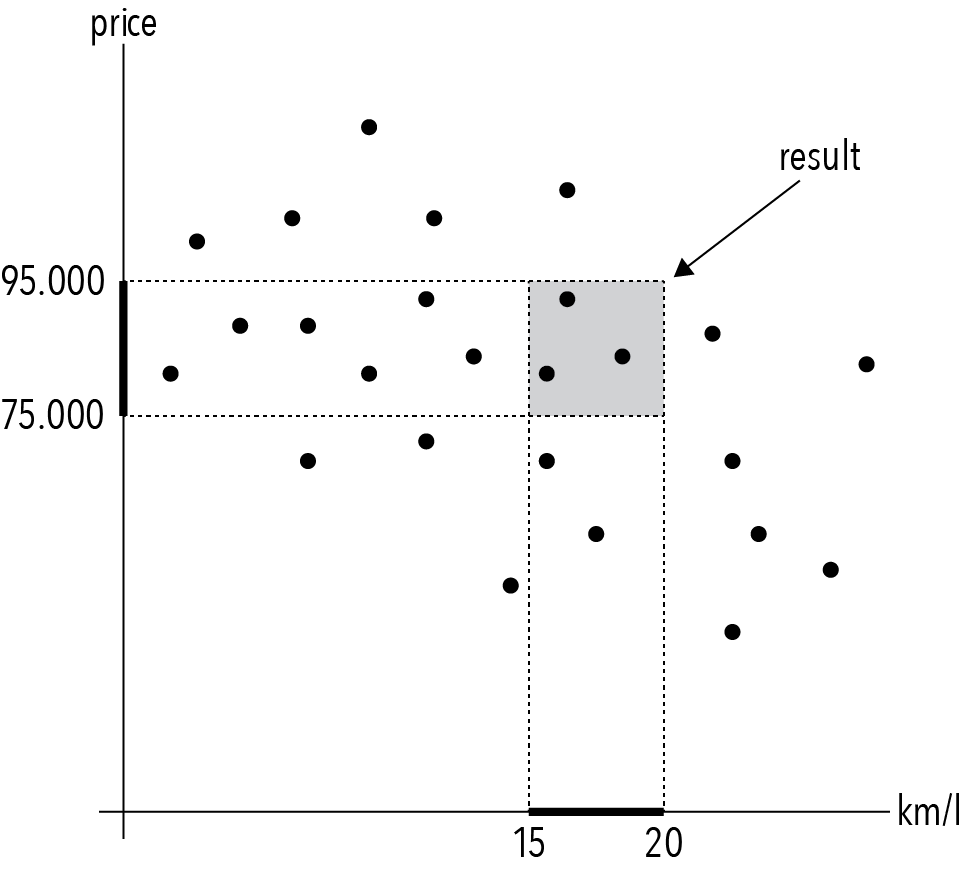
\includegraphics[scale=0.8]{pictures/introduction.png}
    \end{center}
    \column{0.3\textwidth}
    Punkter repræsenterer objekter der er plottet efter to attributer. Nu kan der søges.\\

    Opdeling af akser.


  \end{columns}

\end{frame}

\begin{frame}{Preleminaries}
  \frametitle{Preleminaries}
  Orthogonal range searching
  \begin{itemize}
    \item Svar effektivt på forespørgslen $q = [x_1, x_2] \times [y_1, y_2]$.
    \item $p \in [x_1, x_2] \times [y_1, y_2] \Leftrightarrow p_x \in [x_1, x_2] \wedge p_y \in [y_1, y_2]$
  \end{itemize}

  Preleminaries
  \begin{itemize}

    \item $n$ punkter fra $\mathbb{R}^2$. Alle koordinater er unikke
    \item Rank space. Sorteret array. Vi finder $\hat{y}_1$ og $\hat{y}_2$ og så ved vi hvor mange elementer der er imellem dem.
    \item $n$ er en potens af $2$
    \item static og output-sensitive
  \end{itemize}
\end{frame}

\subsection{kd-tree}

\begin{frame}{kd-træ}
  \frametitle{kd-træ}
  Jon L. Bentley. 1975.
  \begin{itemize}
    \item $\mathcal{O}(n)$ plads
    \item $\mathcal{O}(\sqrt{n} + k)$ tid
  \end{itemize}

  Givet $n$ punkter: $x$ eller $y$ på skift. Et punkt per blad i træet.
\end{frame}

\begin{frame}{Opbygning}
  \frametitle{Opbygning af kd-træ}
  Det $\lceil \frac{n}{2} \rceil$'te element bliver valgt som median. Dette element fungerer som en skille-linje mellem de to punkt-mængder. 
  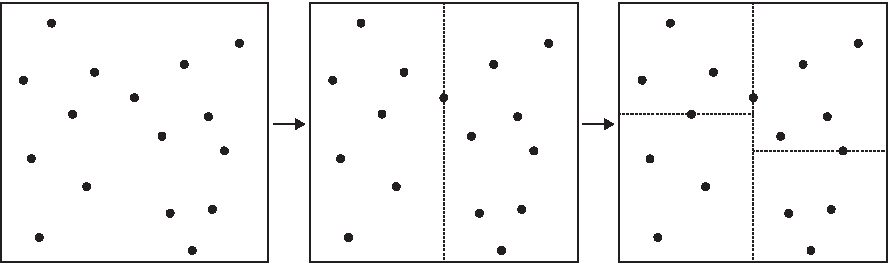
\includegraphics[scale=0.75]{pictures/kd_subdivision-eps-converted-to.pdf}

    Punkter i region, punkter i undertræ. Under-opdel.
\end{frame}


\begin{frame}{Søgning}
  \frametitle{Søgning i kd-træ}
  \begin{center}
    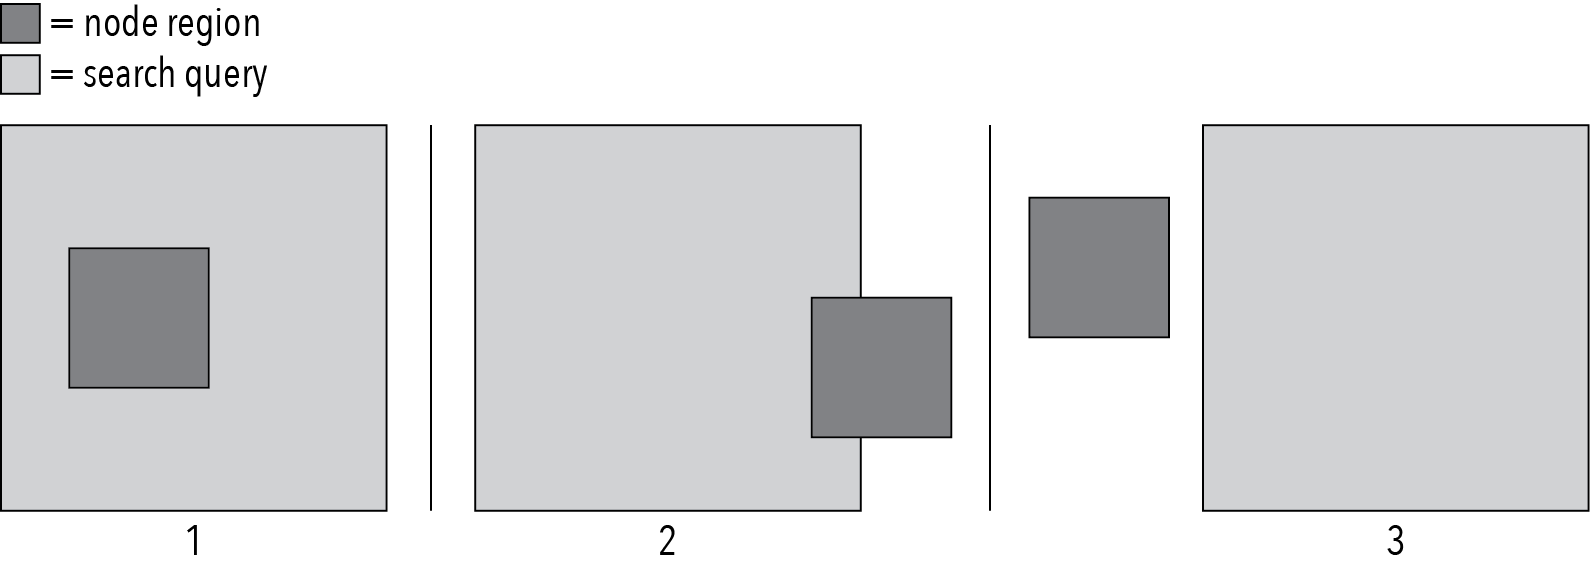
\includegraphics[scale=0.75]{pictures/search_query_overlap.png} \\

    $1$ tager $\mathcal{O}(k)$ tid, $3$ tager $\mathcal{O}(1)$ tid. Bound på $2$.\\


  \end{center}

\end{frame}


\begin{frame}{Søgning}
  \frametitle{Søgning i kd-træ}
  \begin{columns}
    \column{0.7\textwidth}
  \begin{center}
    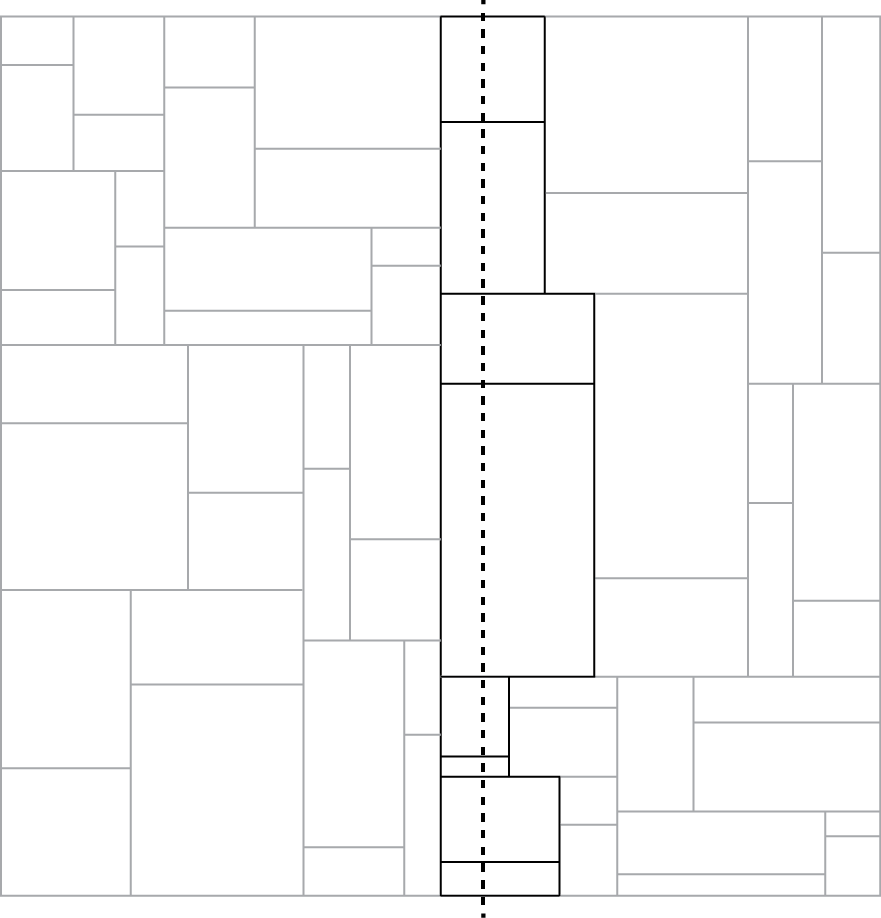
\includegraphics[scale=0.75]{pictures/kd_bound2.png}
  \end{center}
  \column{0.3\textwidth}
  $\mathcal{O}(\sqrt{n})$ regioner.
\end{columns}
\end{frame}


% Section and subsections will appear in the presentation overview
% and table of contents.

\section{Ball Inheritance Search}

\subsection{Ball Inheritance Problem}



\begin{frame}{Ball Inheritance}

  \begin{itemize}
    \item Vi er givet et perfekt binært træ.
      \pause
    \item Roden indeholder $n$ punkter(bolde) som er blevet fordelt sådan at hvert blad lagrer et punkt. Boldene i roden er sorteret.
      \pause
    \item Hver knude har en liste over hvilke bolde der går igennem den. Boldene i knudens liste har samme rækkefølge som boldene i forældre-knudens liste.
     \pause
    \item Løs: Givet en knude og et index i knudens liste, hvilket blad ender denne bold ved?
     \pause
    \item Vi kan nu følge en bold fra en knude til et blad med $\mathcal{O}(\lg n)$ skridt. 

  \end{itemize}
\end{frame}

\begin{frame}{ball inheritance}
  \begin{center}
    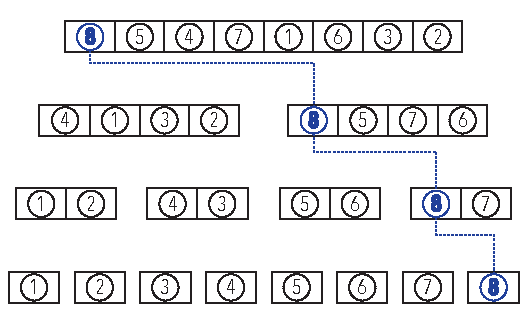
\includegraphics[scale=1.0]{pictures/bolde_8.pdf}
  \end{center}
\end{frame}


\begin{frame}{ball inheritance}
  \begin{center}
    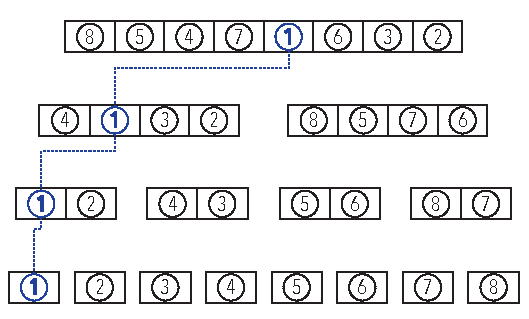
\includegraphics[scale=1.0]{pictures/bolde_1.pdf}
  \end{center}
\end{frame}

\begin{frame}{ball inheritance}
  \begin{center}
    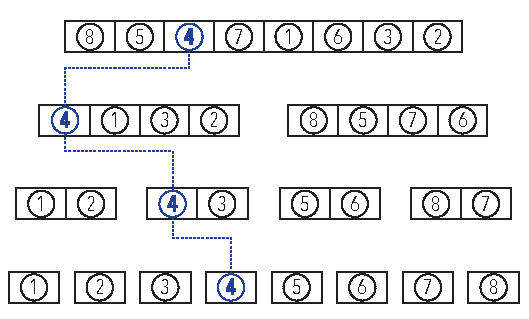
\includegraphics[scale=1.0]{pictures/bolde_4.pdf}
  \end{center}
\end{frame}


\begin{frame}{RANK SELECT}

  Givet en bitvektor, så er Rank-Select query en constant-time query der finder boldens nye position i barnets bitvektor.

  Man kan nu komme ned med $\mathcal{O}(\lg n)$ tid. $\mathcal{O}(1\cdot\lg n)$.
\end{frame}


\begin{frame}{ball inheritance}
  \begin{center}
    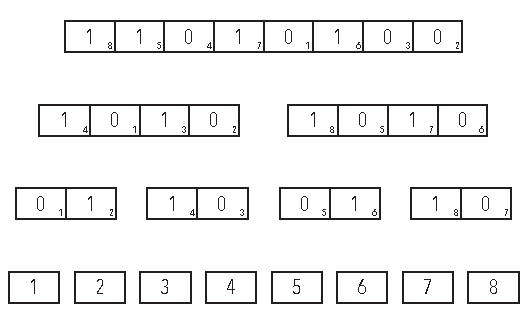
\includegraphics[scale=1.0]{pictures/uden_bolde_med_tal.pdf}
  \end{center}
\end{frame}



\begin{frame}{Faster Queries}
  Færre skridt fra knude til blad. Knuder på niveau deleligt med $B^i$ hopper $B^i$ niveauer over. \\

  Det bruger
  \begin{itemize}
    \item $\mathcal{O}(n \cdot \lg_B \lg n) = \mathcal{O}(\frac{n}{\epsilon}) = \mathcal{O}(n)$ plads
    \item $\mathcal{O}(B \cdot \lg_B \lg n) = \mathcal{O}(\lg^\epsilon n)$ tid
  \end{itemize}
  hvor $\epsilon > 0$ er en arbitrær lille konstant. Space-time tradeoff.\\

  \pause
  $B = \Omega(\lg^\epsilon n)$ og $B = \lg^\frac{\epsilon}{2} = \Omega(\lg \lg n)$.\\

  $\lg_B \lg n$ er valgt fordi $B^i \leq \lg n \Leftrightarrow i \leq \lg_B \lg n$.
\end{frame}

\subsection{Ball Inheritance Search Data Structure}

\begin{frame}{BISintro}
  Ball Inheritance Search (BIS) er en datastruktur som er en simplificering af den datastruktur der findes i \textbf{Orthogonal Range Searching on the RAM, Revisited}\cite{chanetal} af Chan et al.\\

  $\mathcal{O}(\lg n + k\cdot\lg^\epsilon n)$ imod $\mathcal{O}(\lg \lg n + (1+k)\cdot\lg^\epsilon n)$.

\end{frame}


\begin{frame}{Ball Inheritance Search}

  \begin{itemize}
    \item $\mathcal{O}(n + n\cdot\lg_B\lg n) = \mathcal{O}(n + \frac{n}{\epsilon})$ plads.
    \item $\mathcal{O}(\lg n + k\cdot B\lg_B\lg n) = \mathcal{O}(\lg n + k\cdot\lg^\epsilon n)$ tid, hvor $\epsilon > 0$ er en arbitrær lille konstant
  \end{itemize}
    da vi har valgt $B = \Omega(\lg^\epsilon n) = \lceil \frac{1}{2}\lg^\frac{1}{3} n \rceil$.
\end{frame}


\begin{frame}{Ball Inheritance Search}
  Når vi kigger på BIS, så er punkterne \textbf{fordelt} efter x og \textbf{sorteret} efter y. Det betyder
  \begin{itemize}
    \item Undertræer i knuder i mellem $x_1$ og $x_2$ kun indeholder punkter i $[x_1, x_2]$.
    \item Bolde mellem $\hat{y}_1$ og $\hat{y}_2$ kun indeholder punkter i $[y_1, y_2]$.
  \end{itemize}
\end{frame}

\begin{frame}{ball inheritance}
  \begin{center}
    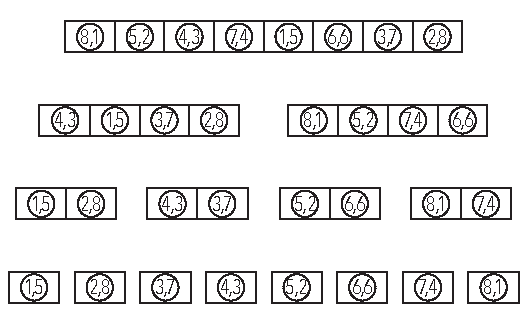
\includegraphics[scale=1.0]{pictures/bolde_med_to_tal.pdf}
  \end{center}
\end{frame}


\begin{frame}{Ball Inheritance Search}
  I denne datastruktur bruger vi ball-inheritance til
  \begin{itemize}
    \item Følge en bold ned når vi ved den ligger i vores søge-område. Dvs dekode fra bold-til-blad(punkt).
    \item Fra roden, opdatere et interval af hvilke bolder der ligger i $[y_1, y_2]$.
  \end{itemize}

  Nu har vi markeret de bolde der ligger i $[y_1, y_2]$ på de knuder hvis undertræ kun indeholder punkter i $[x_1, x_2]$. Og det er netop de punkter der ligger i $[x_1, x_2] \times [y_1, y_2]$.
\end{frame}


\begin{frame}{ball inheritance}
  \begin{center}
    \begin{columns}
      \column{0.5\textwidth}
        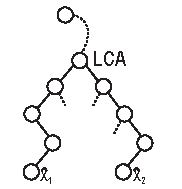
\includegraphics[scale=1.5]{pictures/BIS.pdf}
      \column{0.5\textwidth}
        \begin{itemize}
          \item Rank space opslag ved roden.
          \item Vedligehold $[\hat{y}_1, \hat{y}_2]$ ned til LCA.
          \item Find fully contained knuder og deres $[\hat{y}_1, \hat{y}_2]$ interval.
          \item Ball Inheritance fra knuder.
        \end{itemize}
      \end{columns}
  \end{center}
\end{frame}

\begin{frame}{Ball Inheritance Search}

  Vi har nu nogle knuder og lister over indeces i disse knuder. Det er præcis det problem ball inheritance løser. Vi kan nu bruge ball inheritance på alle disse knuder til at finde ud af hvilke blade der indeholder punkter i $[y_1, y_2]$.

  Det giver en kørselstid på $\mathcal{O}(\lg n + k\cdot\lg^\epsilon n)$ for at finde $k$ punkter.

\end{frame}

\begin{frame}{plads}
  Denne datastruktur bruger $\mathcal{O}(n)$ plads.
  \begin{itemize}
    \item Bit vectors. $\mathcal{O}(n)$ bits per level.
      \pause
    \item Store hop $\mathcal{O}(\lg \Sigma)$ bits per entry hvert $\lg \Sigma$ level. ($\lg \Sigma = B^i$).
      \pause
    \item Egentlig punkter
      \pause
    \item Binær søgning
  \end{itemize}
\end{frame}


\section{Resultater}
\subsection{Resultater}

\begin{frame}{setup}
  \begin{itemize}
    \item Square area $\sqrt{n}\cdot\sqrt{k}\times\sqrt{n}\cdot\sqrt{k}$ returnerer $k$ punkter.
    \item Slices af størrelse $k$ returnerer $k$ punkter. $[0,n] \times [y, y+k]$
    \item $\sqrt{n}+k = \lg n + k\cdot\lg^\epsilon n \Leftrightarrow k = \frac{\sqrt{n}-\lg n}{\lg^\epsilon n -1}$
  \end{itemize}
\end{frame}

\begin{frame}
      \begin{itemize}
        \item $\mathcal{O}(\lg n + k\cdot\lg^\epsilon n)$ vs $\mathcal{O}(\sqrt{n} + k)$.
        \item BIS er mere stabil når vi ændrer shape. $\mathcal{O}(\sqrt{n})$ er problemet.
        \item Slice er godt for BIS og square er godt for kd-træ.
        \item kd-træ er hurtigere jo flere punkter, og jo mindre $\mathcal{O}(\sqrt{n})$ er.
        \item $\lg n < \sqrt{n}$, så vi forventer at en dårlig shape betyder meget for kd-træet.
        \item Vi har også kigget på $k \leq 200$ for personlig interaktion. Der er BIS god.
      \end{itemize}
\end{frame}

\begin{frame}{Squared}
  \begin{columns}
    \column{0.5\textwidth}
    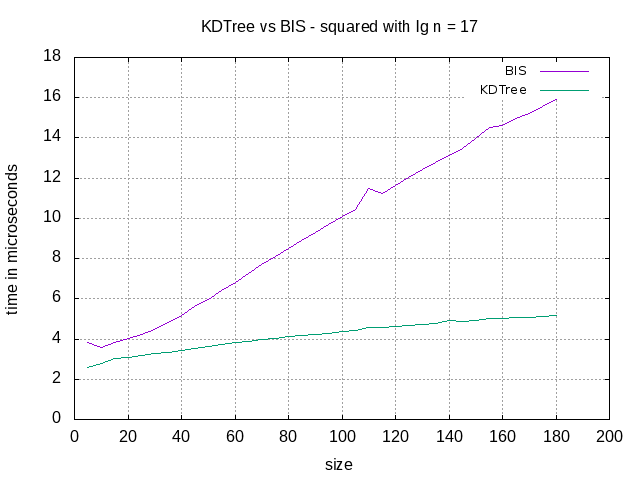
\includegraphics[scale=0.32]{pictures/analysis/sqrt_17.png}
    \column{0.5\textwidth}
    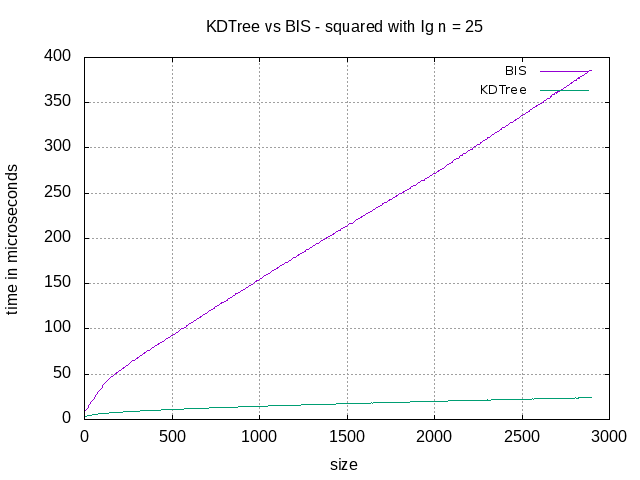
\includegraphics[scale=0.32]{pictures/analysis/sqrt_25.png}
  \end{columns}
\end{frame}

\begin{frame}{Squared}

  \begin{center}
    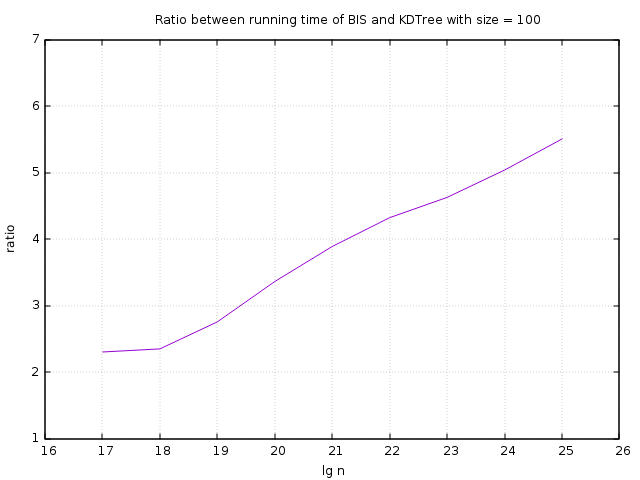
\includegraphics[scale=0.35]{pictures/analysis/factor_difference_sqrtn_100.png}
  \end{center}

\end{frame}

\begin{frame}{vertical}
  \begin{columns}
    \column{0.5\textwidth}
    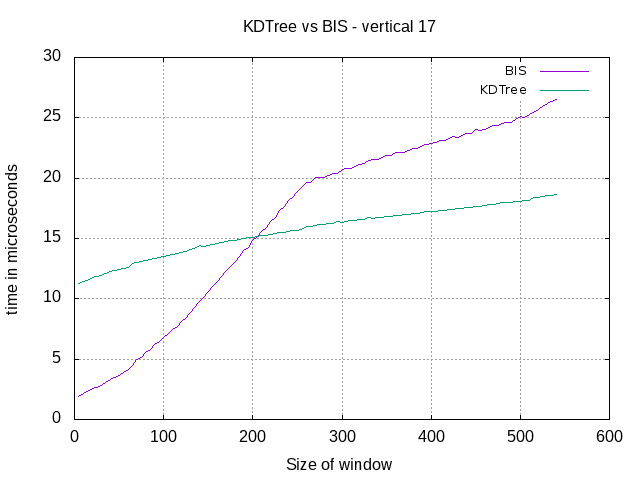
\includegraphics[scale=0.32]{pictures/analysis/vert_17.png}
    \column{0.5\textwidth}
    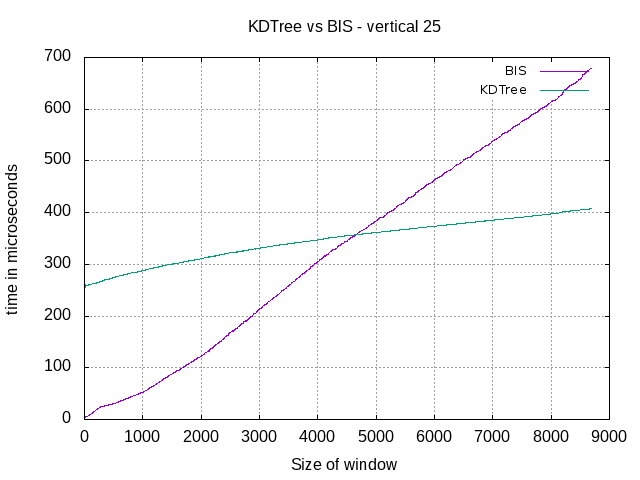
\includegraphics[scale=0.32]{pictures/analysis/vert_25.png}
  \end{columns}
\end{frame}

\begin{frame}{vertical}
  \begin{columns}
    \column{0.5\textwidth}
    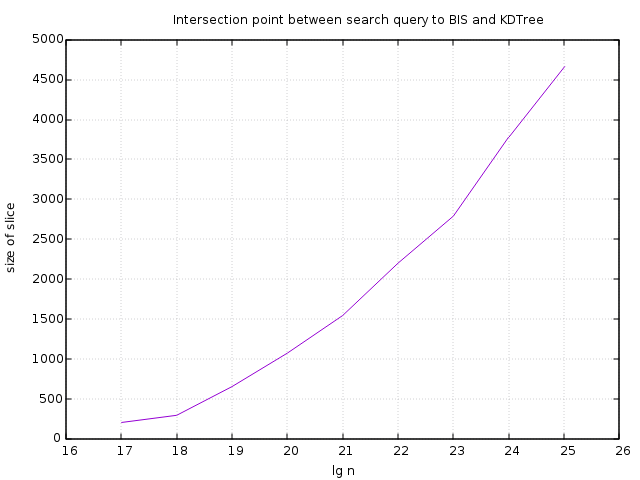
\includegraphics[scale=0.3]{pictures/analysis/vert.png}
    \column{0.5\textwidth}
    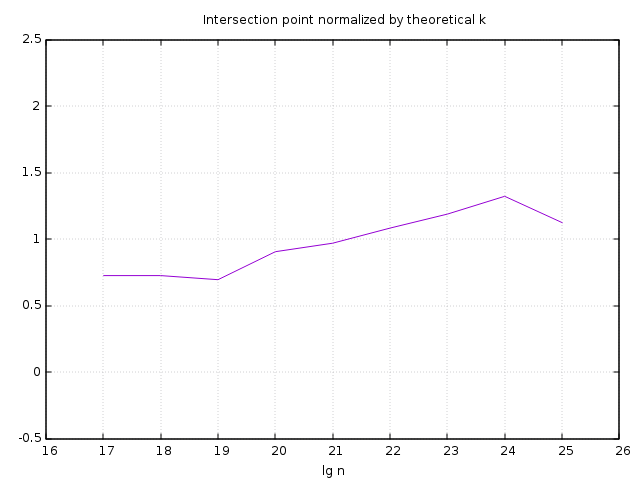
\includegraphics[scale=0.3]{pictures/analysis/vert_theory.png}
  \end{columns}
\end{frame}

\begin{frame}{horizontal}
  \begin{columns}
    \column{0.5\textwidth}
    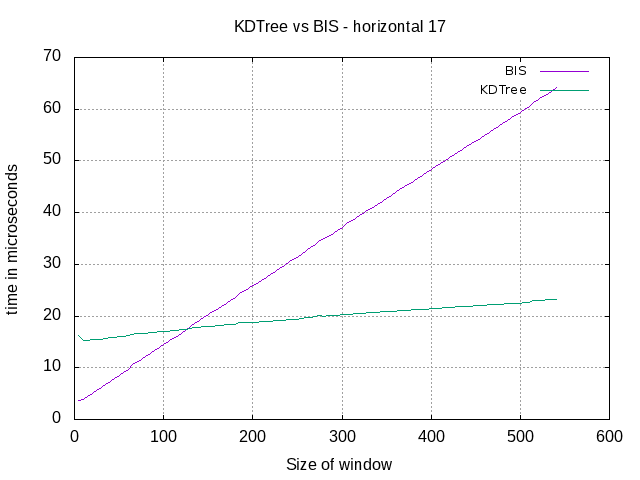
\includegraphics[scale=0.34]{pictures/analysis/hori_17.png}
    \column{0.5\textwidth}
    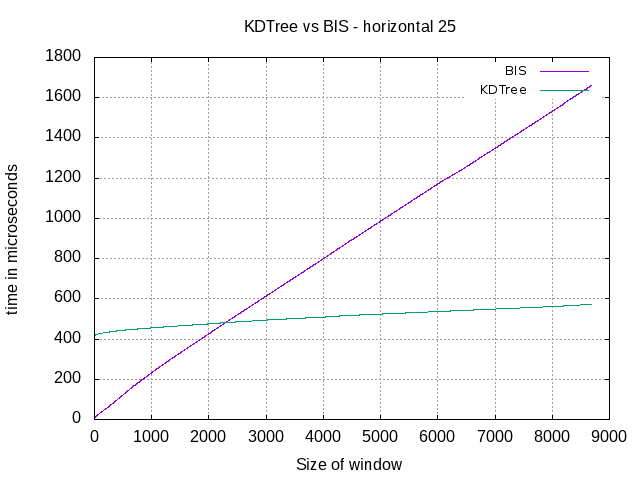
\includegraphics[scale=0.34]{pictures/analysis/hori_25.png}
  \end{columns}
\end{frame}

\begin{frame}{horizontal}
  \begin{columns}
    \column{0.5\textwidth}
    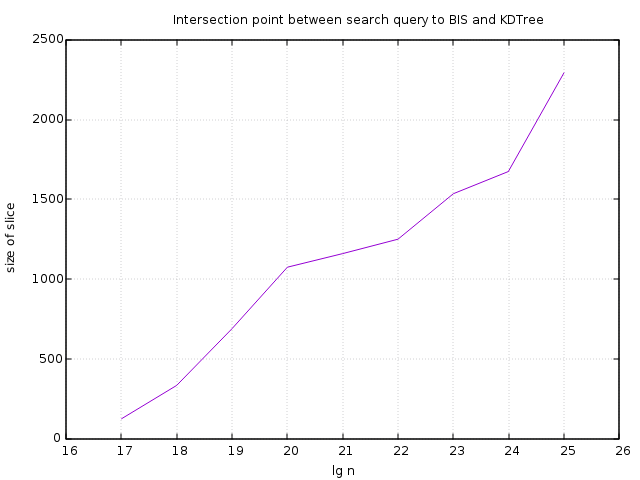
\includegraphics[scale=0.3]{pictures/analysis/hori.png}
    \column{0.5\textwidth}
    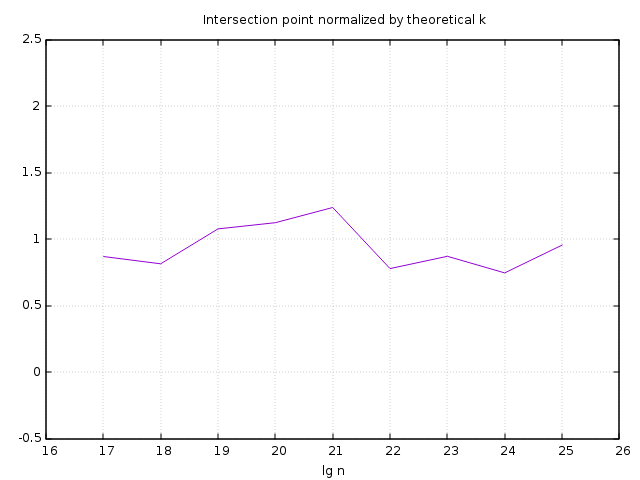
\includegraphics[scale=0.3]{pictures/analysis/hori_theory.png}
  \end{columns}
\end{frame}

\begin{frame}{small k}
  \begin{columns}
    \column{0.5\textwidth}
    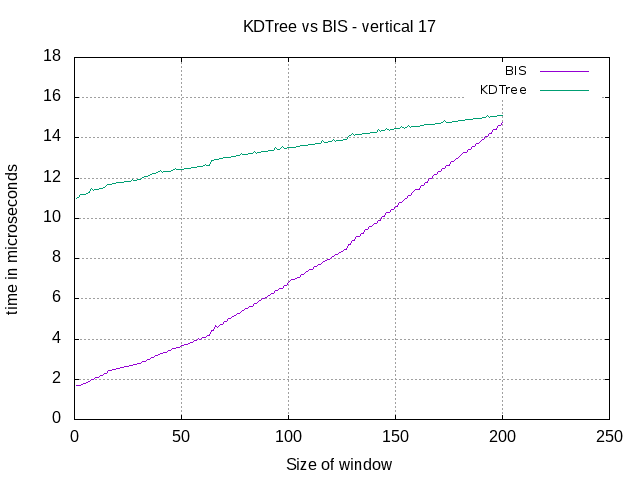
\includegraphics[scale=0.35]{pictures/analysis/smalls/vert_17.png}
    \column{0.5\textwidth}
    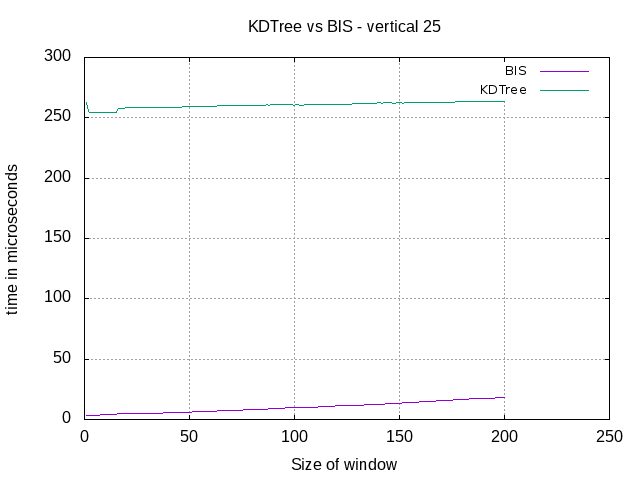
\includegraphics[scale=0.35]{pictures/analysis/smalls/vert_25.png}
  \end{columns}
\end{frame}

\begin{frame}{small k}
  \begin{columns}
    \column{0.5\textwidth}
    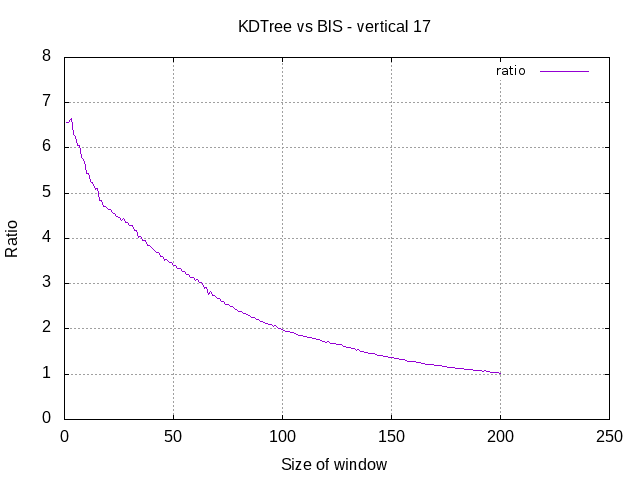
\includegraphics[scale=0.35]{pictures/analysis/smalls/vert_fac_17.png}
    \column{0.5\textwidth}
    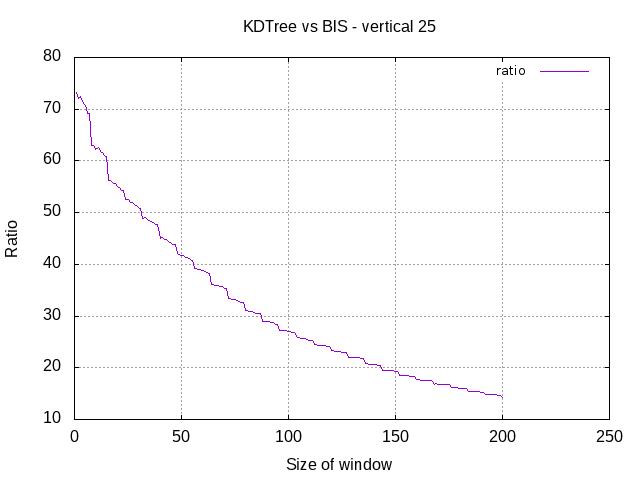
\includegraphics[scale=0.35]{pictures/analysis/smalls/vert_fac_25.png}
  \end{columns}
\end{frame}


\begin{frame}{small k}
  \begin{columns}
    \column{0.5\textwidth}
    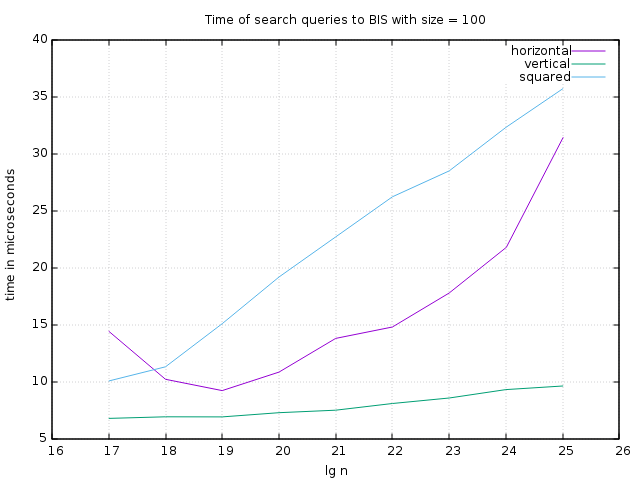
\includegraphics[scale=0.32]{pictures/analysis/smalls/all_100.png}
    \column{0.5\textwidth}
    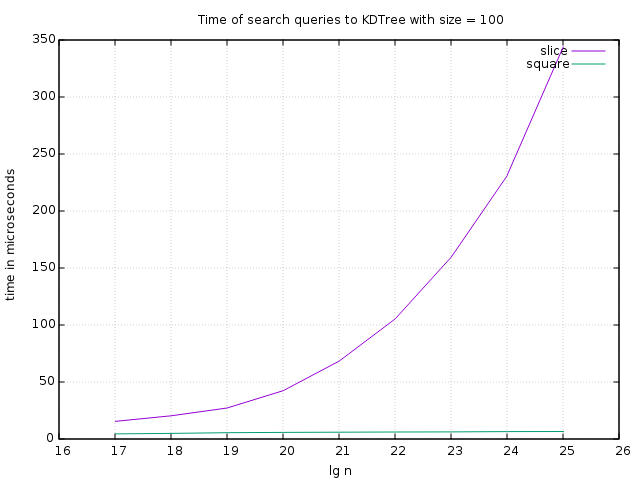
\includegraphics[scale=0.32]{pictures/analysis/smalls/all_kdtree_100_2.png}
  \end{columns}
\end{frame}

\begin{frame}{small k}
  \begin{columns}
    \column{0.5\textwidth}
    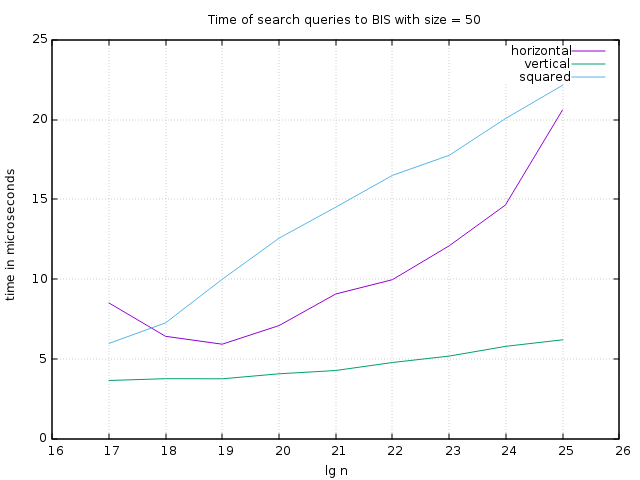
\includegraphics[scale=0.32]{pictures/analysis/smalls/all_50.png}
    \column{0.5\textwidth}
    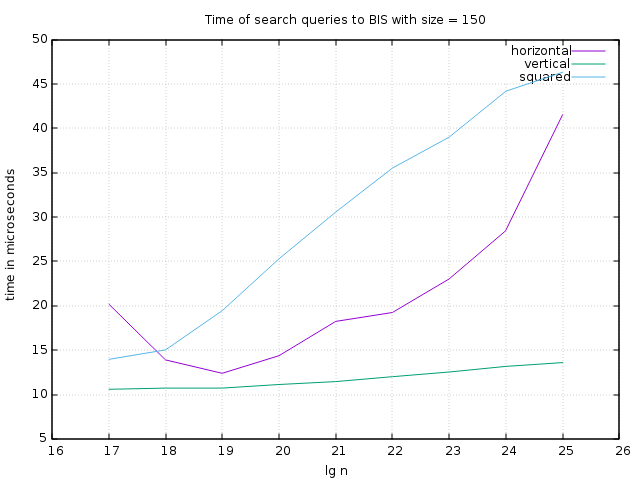
\includegraphics[scale=0.32]{pictures/analysis/smalls/all_150.png}
  \end{columns}
\end{frame}

\begin{frame}{small k}
  \begin{columns}
    \column{0.5\textwidth}
    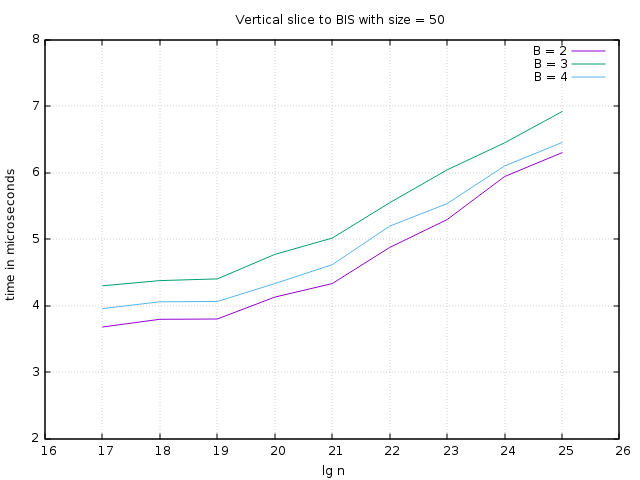
\includegraphics[scale=0.32]{pictures/analysis/comparing_BIS_50.png}
    \column{0.5\textwidth}
    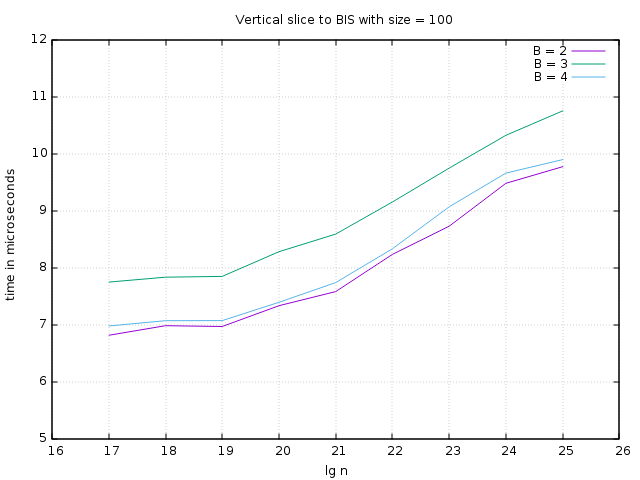
\includegraphics[scale=0.32]{pictures/analysis/comparing_BIS_100.png}
  \end{columns}
\end{frame}

\begin{frame}{sizes}
  \begin{center}
    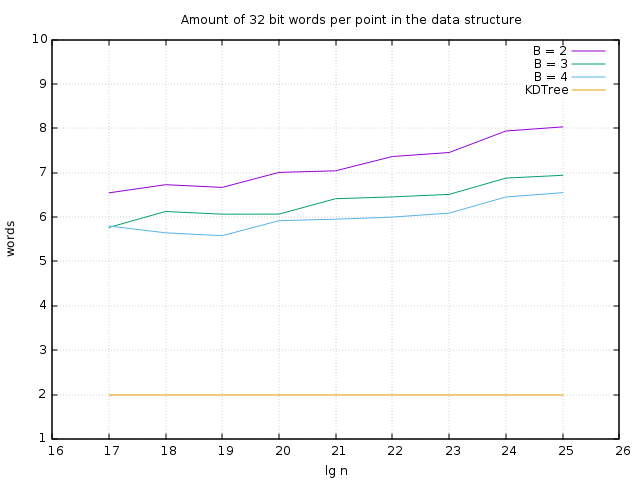
\includegraphics[scale=0.35]{pictures/analysis/sizes.png}
  \end{center}
\end{frame}

\begin{frame}{Future work}
  \begin{itemize}
    \item Bedre udpakning
    \item Cache
    \item Concurrency
  \end{itemize}
\end{frame}

\begin{frame}{Færdig}
  Spørgsmål?
\end{frame}


\begin{frame}{praktisk log epsilon n}
  \begin{center}
    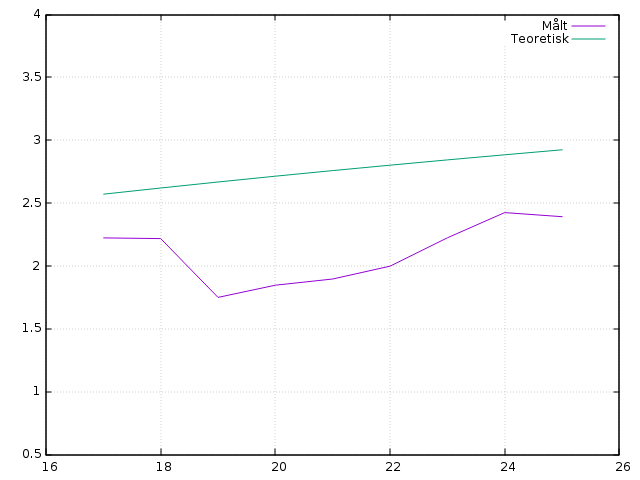
\includegraphics[scale=0.35]{pictures/theory_vs_actual.png}
  \end{center}
\end{frame}


\begin{frame}{Små hop}
  Hvert niveau gemmer $n$ bits som indikerer om bolden er gået til højre eller venstre. Hvert $32$ bit gemmer vi et $32$ bit major checkpoint. Precomputed tabel med $16$ bit tal som tæller antal $1$-entries. $\mathcal{O}(n)$ bits per level.
\end{frame}

\begin{frame}{Store hop}
  $\mathcal{O}(\lg \Sigma)$ per entry. $\Sigma = 2^{B^i}$. Så plads er $\mathcal{O}(B^i)$ bits per entry.\\

  Det er $$\sum_{i=1}^{\lg_B \lg n} \frac{\lg n}{B^i}\cdot\mathcal{O}(B^i) = \mathcal{O}(\lg n \cdot \lg_B \lg n)$$ for hele kæden. Vælg nu $B = \Omega(\lg^\epsilon n)$.


  Vi har $n$ punkter, hvilket giver $\mathcal{O}(n\lg n \cdot\lg_B \lg n)$ bits. Det er $\mathcal{O}(n\cdot\frac{\lg lg n}{\epsilon \lg \lg n}) = \mathcal{O}(\frac{n}{\epsilon})$ ord.
\end{frame}

\begin{frame}{Store hop}
  Tiden for de store hop er højst $\mathcal{O}(B \lg_B \lg n)$. Vælg $B = \lg^{\epsilon / 2} n = \Omega(\lg \lg n)$.
\end{frame}


\begin{frame}{OBIS}
  OBIS af Chan et al. Med $\mathcal{O}(n)$ plads og $\mathcal{O}(\lg \lg n + (1+k)\cdot\lg^\epsilon n)$. Bruger også Ball Inheritance til at finde de $k$ punkter.
\end{frame}

\begin{frame}{OBIS}
  \begin{columns}
    \column{0.5\textwidth}
    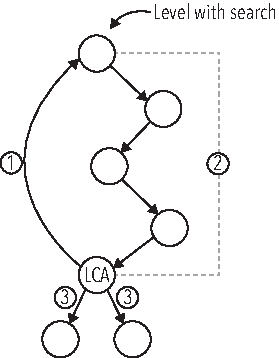
\includegraphics{pictures/ors_step2-eps-converted-to.pdf}
    \column{0.5\textwidth}
    \begin{itemize}
      \item Op til nærmeste level med pred-search
      \item Gå ned til LCA højst $\lg \lg n$ levels nede.
      \item Gå ned og find resultater i begge børn af LCA.
    \end{itemize}

  \end{columns}
\end{frame}

\begin{frame}{OBIS}

  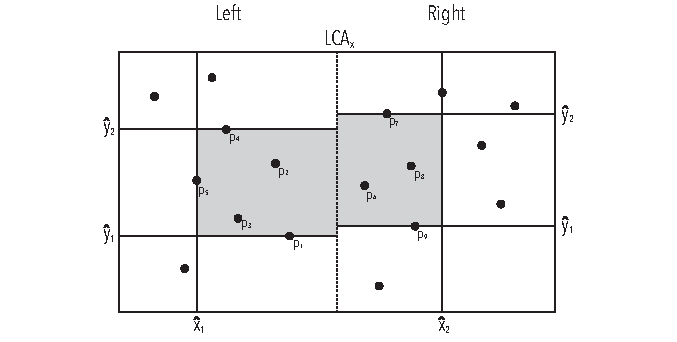
\includegraphics{pictures/ors_step3-eps-converted-to.pdf}
\end{frame}




\begin{frame}{small k}
  \begin{columns}
    \column{0.5\textwidth}
    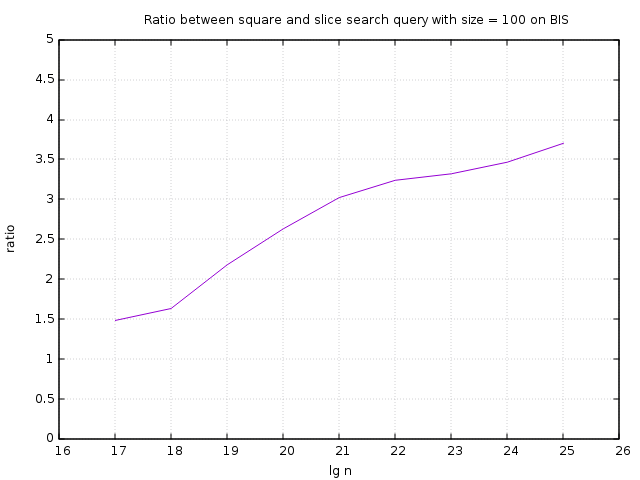
\includegraphics[scale=0.32]{pictures/analysis/smalls/bis_ratio_100.png}
    \column{0.5\textwidth}
    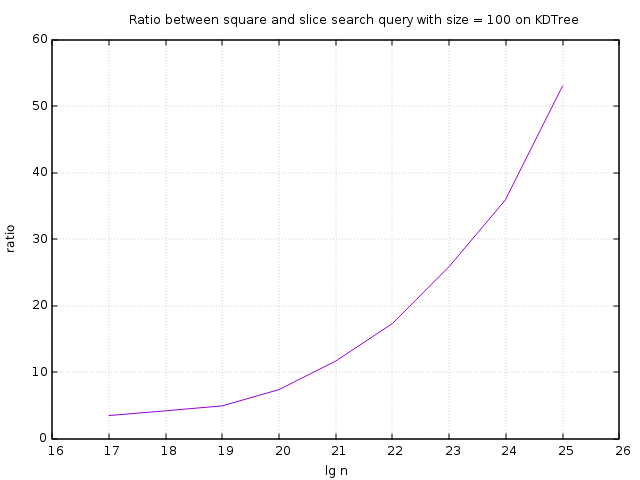
\includegraphics[scale=0.32]{pictures/analysis/smalls/kdtree_ratio_100.png}
  \end{columns}
\end{frame}



\begin{frame}[allowframebreaks]
  \frametitle<presentation>{References}
    
  \begin{thebibliography}{10}
    
  \beamertemplatebookbibitems
  % Start with overview books.

  \bibitem{chanetal}
    Timothy M. Chan, Kasper Green Larsen, Mihai Patrascu.
    \newblock {\em Orthogonal Range Searching on the RAM, Revisited}.
 \end{thebibliography}
\end{frame}

\end{document}


